\documentclass[11pt,a4paper]{article}
\usepackage[pdftex]{color,graphicx}
\usepackage{tabularx}

% Uncomment the following two lines to check syntax only (no .dvi output produced, so it's faster!)
%\usepackage{syntonly}
%\syntaxonly

%\pagestyle{headings}

% Superscript and subscript commands
\newcommand{\superscript}[1]{\ensuremath{^{\textnormal{\scriptsize{#1}}}}}
\newcommand{\subscript}[1]{\ensuremath{_{\textnormal{\scriptsize{#1}}}}}

% Define the title
\title{FmcAdc100m14b4cha User's Guide}
\author{Matthieu Cattin}

\begin{document}

% Insert logos
\begin{figure}[t]
  
\includegraphics[height=3cm]{figures/cern_logo.pdf}
  \label{fig:cern_logo}
  \hfill
  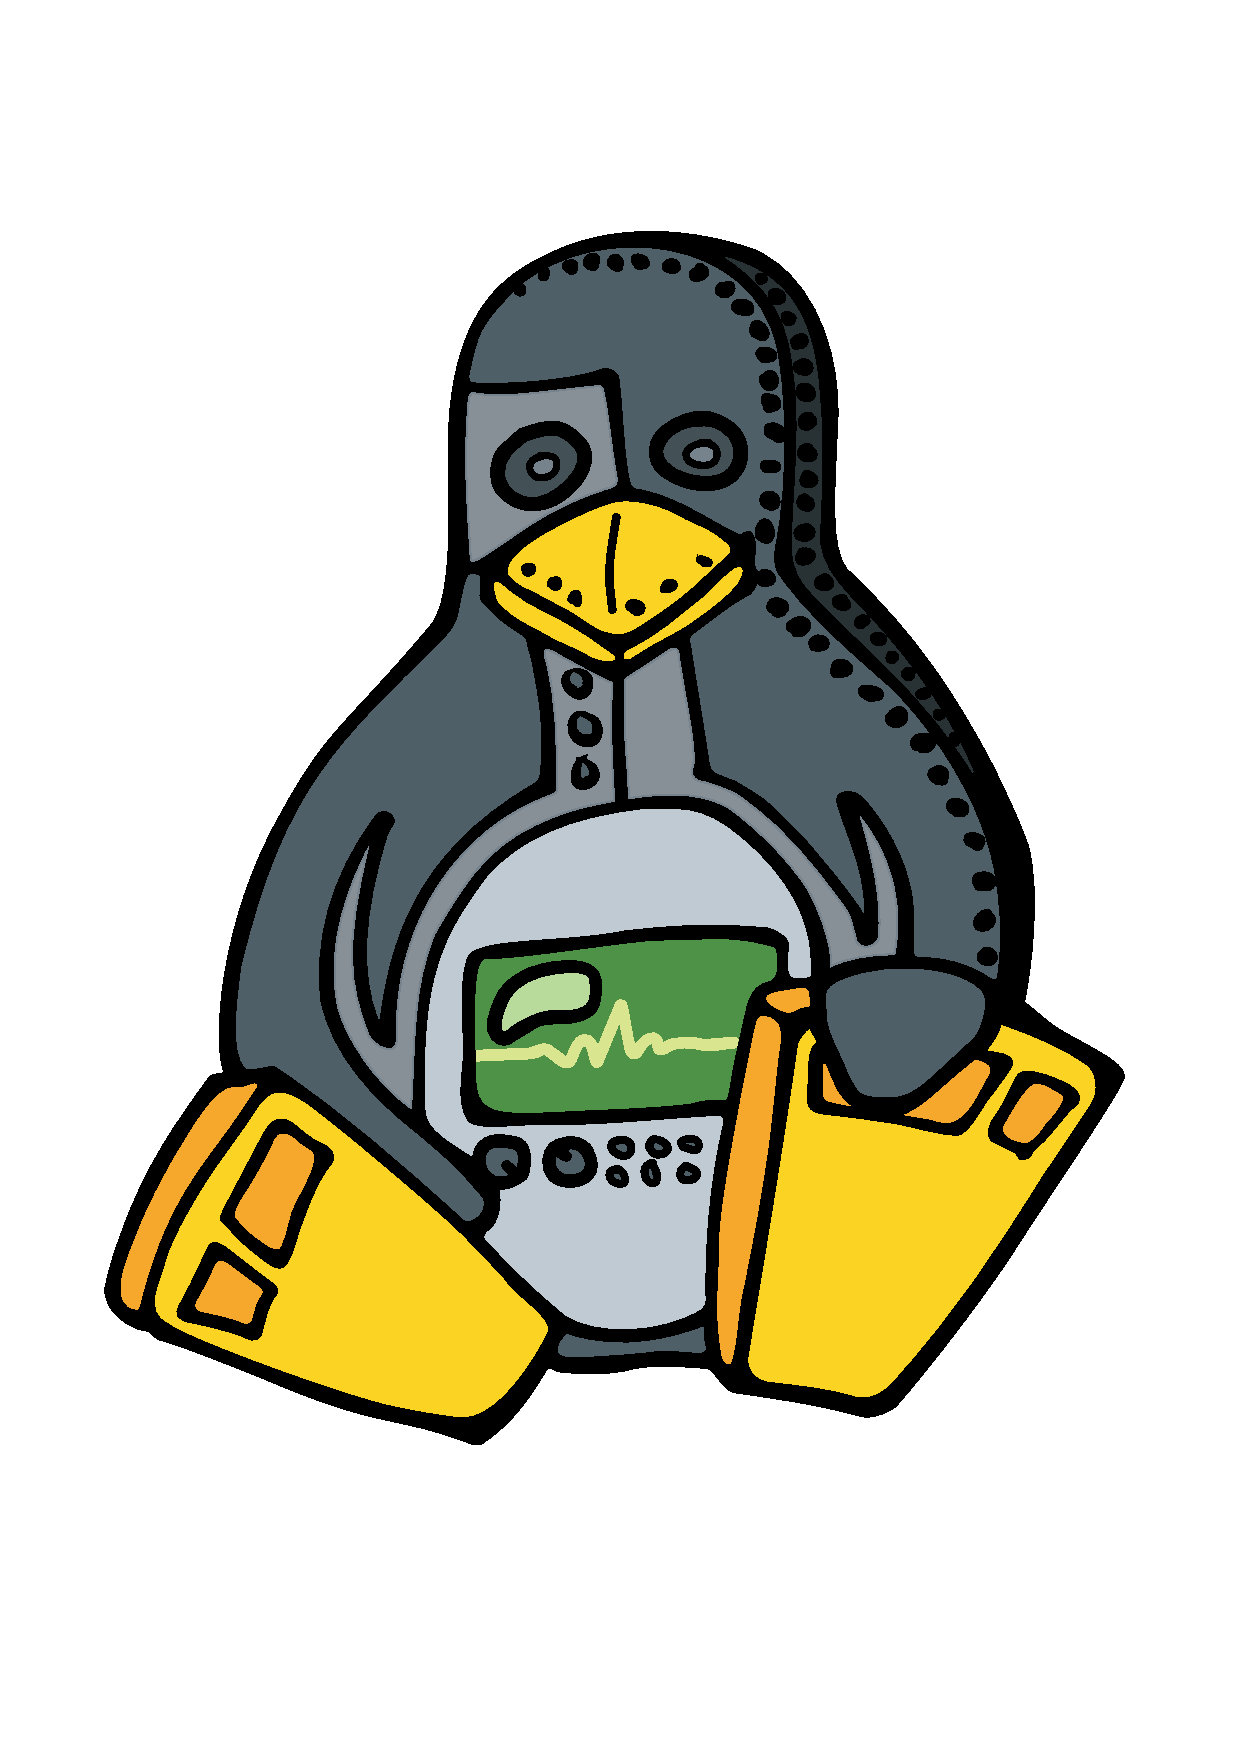
\includegraphics[height=3cm]{figures/ohr_logo.pdf}
  \label{fig:ohr_logo}
\end{figure}

% Generate the title
\maketitle

% Document abstract
\begin{abstract}
This document, blabla...
\end{abstract}


% Revision history
\newpage
\begin{tabularx}{1.0\textwidth}{| c | c | l | X |}
\hline
Revision & Date & Author &  Comments\\
\hline
0.1 & 07.02.2012 & Matthieu CATTIN & Initial revision\\
\hline
\end{tabularx}

% Insert a table of content
\newpage
\tableofcontents

% Start sections on a new page
\newpage

%===============================================================================
\section{Overview}
Here's an overview of the fmcadc100m14b4cha board...

%===============================================================================
\section{Acquisition}

* Single shot mode:


* Multi-shot mode:


\subsection{Trigger}


\subsection{Memory}


\section{Calibration}

The calibration is done once during the prodoction tests.
It can be repeated afterwards with the production test suite (PTS) and the corresponding testbench.
The calibration process gives four values per channel and per input range:
ADC gain correction, ADC offset correction, DAC gain correction and DAC offset correction.
The temperature during the calibration process is also measured.
All the calibration values are stored in the FmcAdc100m14b4cha EEPROM.
Tables \ref{tab:adc_calibr_data_eeprom} and \ref{tab:dac_calibr_data_eeprom} shows the calibration data types and the arrangement in the EEPROM.
Note that ADC calibration data are stored before DAC calibration data in the EEPROM.

\begin{table}[ht]
  \centering
  \begin{tabularx}{\textwidth}{|c|l|X|}
    \hline
    \multicolumn{3}{|c|}{\textbf{ADC correction values}} \\ \hline
    \textbf{Input range}  & \textbf{Description} & \textbf{Type} \\ \hline
    10V & Offset correction channel 1 & 16-bit signed \\
    & Offset correction channel 2 & 16-bit signed \\
    & Offset correction channel 3 & 16-bit signed \\
    & Offset correction channel 4 & 16-bit signed \\
    \cline{2-3}
    & Gain correction channel 1 & 16-bit unsigned \\
    & Gain correction channel 2 & 16-bit unsigned \\
    & Gain correction channel 3 & 16-bit unsigned \\
    & Gain correction channel 4 & 16-bit unsigned \\
    \cline{2-3}
    & Temperature & 16-bit unsigned * 0.01$^\circ$C \\
    \hline
    1V & Offset correction channel 1 & 16-bit signed \\
    & Offset correction channel 2 & 16-bit signed \\
    & Offset correction channel 3 & 16-bit signed \\
    & Offset correction channel 4 & 16-bit signed \\
    \cline{2-3}
    & Gain correction channel 1 & 16-bit unsigned \\
    & Gain correction channel 2 & 16-bit unsigned \\
    & Gain correction channel 3 & 16-bit unsigned \\
    & Gain correction channel 4 & 16-bit unsigned \\
    \cline{2-3}
    & Temperature & 16-bit unsigned * 0.01$^\circ$C \\
    \hline
    100mV & Offset correction channel 1 & 16-bit signed \\
    & Offset correction channel 2 & 16-bit signed \\
    & Offset correction channel 3 & 16-bit signed \\
    & Offset correction channel 4 & 16-bit signed \\
    \cline{2-3}
    & Gain correction channel 1 & 16-bit unsigned \\
    & Gain correction channel 2 & 16-bit unsigned \\
    & Gain correction channel 3 & 16-bit unsigned \\
    & Gain correction channel 4 & 16-bit unsigned \\
    \cline{2-3}
    & Temperature & 16-bit unsigned * 0.01$^\circ$C \\
    \hline
  \end{tabularx}
  \caption{ADC calibration data}
  \label{tab:adc_calibr_data_eeprom}
\end{table}

\begin{table}[ht]
  \centering
  \begin{tabularx}{\textwidth}{|c|l|X|}
    \hline
    \multicolumn{3}{|c|}{\textbf{DAC correction values}} \\ \hline
    \textbf{Input range}  & \textbf{Description} & \textbf{Type} \\ \hline
    10V & Offset correction channel 1 & 16-bit signed \\
    & Offset correction channel 2 & 16-bit signed \\
    & Offset correction channel 3 & 16-bit signed \\
    & Offset correction channel 4 & 16-bit signed \\
    \cline{2-3}
    & Gain correction channel 1 & 16-bit unsigned \\
    & Gain correction channel 2 & 16-bit unsigned \\
    & Gain correction channel 3 & 16-bit unsigned \\
    & Gain correction channel 4 & 16-bit unsigned \\
    \cline{2-3}
    & Temperature & 16-bit unsigned * 0.01$^\circ$C \\
    \hline
    1V & Offset correction channel 1 & 16-bit signed \\
    & Offset correction channel 2 & 16-bit signed \\
    & Offset correction channel 3 & 16-bit signed \\
    & Offset correction channel 4 & 16-bit signed \\
    \cline{2-3}
    & Gain correction channel 1 & 16-bit unsigned \\
    & Gain correction channel 2 & 16-bit unsigned \\
    & Gain correction channel 3 & 16-bit unsigned \\
    & Gain correction channel 4 & 16-bit unsigned \\
    \cline{2-3}
    & Temperature & 16-bit unsigned * 0.01$^\circ$C \\
    \hline
    100mV & Offset correction channel 1 & 16-bit signed \\
    & Offset correction channel 2 & 16-bit signed \\
    & Offset correction channel 3 & 16-bit signed \\
    & Offset correction channel 4 & 16-bit signed \\
    \cline{2-3}
    & Gain correction channel 1 & 16-bit unsigned \\
    & Gain correction channel 2 & 16-bit unsigned \\
    & Gain correction channel 3 & 16-bit unsigned \\
    & Gain correction channel 4 & 16-bit unsigned \\
    \cline{2-3}
    & Temperature & 16-bit unsigned * 0.01$^\circ$C \\
    \hline
  \end{tabularx}
  \caption{DAC calibration data}
  \label{tab:dac_calibr_data_eeprom}
\end{table}

Two registers per channel are implemented in the FPGA for ADC gain and offset correction.
When an input range is selected, the corresponding gain/offset correction values must be loaded from the EEPROM to those registers.

As the DAC value is set once before an acquisition, there is no need to implement the gain and offset correction in the FPGA.
Therefore gain and offset correction must be applied to the DAC value by the software.

Below is the pseudo-code to calculate the DAC corrected value, applying gain and offset correction:
\begin{verbatim}
c_val = ((((val-0x8000+offset) << 15) * gain) >> 30)+0x8000
\end{verbatim}







\end{document}
